\documentclass[letterpaper]{article}

% Parts of the style depend on whether a PDF or a DVI output is created.
\usepackage{ifpdf}

\usepackage{aaai}
\usepackage{amsfonts}
\usepackage{amsmath}
\usepackage{amsthm}
\usepackage{courier}
\usepackage[english]{babel}

% Include graphics.
\usepackage{graphicx}
\ifpdf
  % Declare the supported file extensions.
  \DeclareGraphicsExtensions{.jpg,.mps,.pdf,.png}
\fi

\usepackage{helvet}
\usepackage[utf8]{inputenc}
\usepackage{times}
\usepackage{verbatim}

% Operator macros.
\newcommand{\absolute}[1]{\lvert#1\rvert}
\newcommand{\bigsetdef}[2]{\big\{#1\,\,\big\vert\,\,#2\big\}}
\newcommand{\card}[1]{\lvert#1\rvert}
\newcommand{\equivpair}[2]{#1 \approx #2}
\newcommand{\equivset}[1]{[#1]_{\approx}}
\newcommand{\higherapprox}[0]{\overline{\approx}}
\newcommand{\interp}[1]{#1^{\mathcal{I}}}
\newcommand{\lowerapprox}[0]{\underline{\approx}}
\newcommand{\natnum}[1]{#1 \in \mathbb{N}}
\newcommand{\pair}[2]{\langle#1,#2\rangle}
\newcommand{\powerset}[1]{\mathcal{P}{#1}}
\newcommand{\range}[2]{#1,\ldots,#2}
\newcommand{\set}[1]{\{#1\}}
\newcommand{\setdef}[2]{\{#1\,\vert\,#2\}}
\newcommand{\setrange}[2]{\{#1,\ldots,#2\}}
\newcommand{\triple}[3]{\langle#1,#2,#3\rangle}
\newcommand{\tuple}[1]{\langle#1\rangle}
\newcommand{\tuplerange}[2]{\langle#1,\ldots,#2\rangle}

% Operator declarations
\DeclareMathOperator{\indpo}{{\mathbb{IND}-\mathbb{PO}}}
\DeclareMathOperator{\indp}{{\mathbb{IND}-\mathbb{P}}}

% Theorem styles.
\newtheorem{assumption}{Assumption}
\newtheorem{axiom}{Axiom}
\newtheorem{convention}{Convention}
\newtheorem{example}{Example}
\newtheorem{definition}{Definition}
\newtheorem{lemma}{Lemma}
\newtheorem{principle}{Principle}
\newtheorem{proposition}{Proposition}
\newtheorem{specification}{Specification}
\newtheorem{statement}{Statement}
\newtheorem{theorem}{Theorem}
%\theoremstyle{definition}

\frenchspacing

\setlength{\pdfpagewidth}{8.5in}
\setlength{\pdfpageheight}{11in}

\pdfinfo{
/Title Rough Set Semantics for Identity on the Web
/Author Wouter Beek, Stefan Schlobach, Frank van Harmelen}
\setcounter{secnumdepth}{1}

\author{
  Wouter Beek \and Stefan Schlobach \and Frank van Harmelen\\
  Vrije Universiteit Amsterdam\\
  De Boelelaan 1081a\\
  1081HV Amsterdam\\
  The Netherlands
}

\title{Rough Set Semantics for Identity on the Web}

\begin{document}

\maketitle
\begin{abstract}
\begin{quote}
Identity relations are at the foundation of the Linked Open Data initiative
  and on the Semantic Web in general.
They allow the interlinking of alternative descriptions of the same thing.
However, many practical uses of \verb|owl:sameAs| are known to violate its
  formal semantics.
We propose a method that assigns meaning to (the subrelations of)
  an identity relation using the predicates of the dataset schema.
Applications of this approach include automated suggestions for
  asserting/retracting identity pairs and quality assessment.
We also describe an experimental design for this approach.
\end{quote}
\end{abstract}

% Section 1: Introduction
\section{Introduction}
\label{sec:introduction}

Identity relations are at the foundation of the Linked Open Data initiative
  and of the Semantic Web in general \cite{BizerCyganiakHeath2007}.
They allow the interlinking of alternative descriptions of the same thing.
However, the traditional notion of identity
  (expressed by
  {\small \texttt{owl:sameAs}} \cite{MotikPaterschneiderGrau2012})
  is often problematic, e.g. when objects are considered the same in some
  contexts but not in others.
The standing practice in such cases is to use weaker relations of relatedness
  (e.g., {\small \texttt{skos:related}} \cite{MilesBechhofer2009}).
Unfortunately, this limits reasoners in drawing inferences.

According to the traditional semantics of the identity relation,
  identical terms can be replaced for one another in all non-modal contexts
  \emph{salva veritate}.
Practical uses of {\small \texttt{owl:sameAs}} are known to violate this
  strict condition
  \cite{HalpinHayes2010,HalpinHayesMccuskerMcguinnessThompson2010}.

The SW is not only a formal model,
  but is also a social component that evolves over time,
  i.e. it is a social machine \cite{Www2013}.
Being a social and symbolic system at the same time,
  meaning on the SW is denoted by its semantics as well as its pragmatics.

\subsection{Research goals}
\label{sec:research_goals}

In developing our approach we have the following research goals:
\begin{enumerate}
\item In an identity relation the pairs all look the same.
      We want to characterize subrelations of an identity relation in terms
      of the predicates that occur in the schema of the dataset.
\item Based on an existing identity relation we want to give semantically
      motivated suggestions for extending/limiting the identity relation.
\item We want to assess the quality of an identity relation based on
      the consistency with which it is applied to the data.
\end{enumerate}


\section{Stating the problem}
\label{sec:stating_the_problem}

Identity is often thought of as having the exact same properies.
This statement is known as the Principle of indiscernibility
(see principle \ref{principle:indiscernibility_of_identicals})
and has been attributed to Leibniz \cite{Forrest2010}.
% According to Forrest2010 this can be found in Gottfried Wilhelm Leibniz,
% Discourse on Metaphysics, section 9.
% There I find the following passage:
% \begin{quote}
% That every individual substance expresses the whole universe
%   in its own manner and that in its full concept is included
%   all its experiences together with all the attendant circumstances
%   and the whole sequence of exterior events.
% \end{quote}

%\small
\begin{principle}[Indiscernibility of identicals]
\label{principle:indiscernibility_of_identicals}
\begin{equation}
    a = b
  \rightarrow
    \forall_{\phi \in \Phi} \phi(a) = \phi(b)\nonumber
\end{equation}
\end{principle}
%\normalsize

\noindent Although the principle provides necessary and sufficient conditions
  for identity, it does not point towards an automated procedure
  for enumerating the extension of the identity relation,
  since due to its circular nature the set of properties includes
  ``being identical to $x$'' (for every resource $x$).
But even though this priciple does not
  allow a positive identification of identity pairs,
  it does provide an exclusion condition,
  namely resources that are known to not share some property
  are also known to not be identical.

\subsection{Generic problems of identity}

Identity poses several problems which are not specific to the SW.
Firstly, identity does not hold across (all) modal contexts,
  allowing Louis Lane to believe that Superman saved her,
  without her knowling that Clark Kent saved here.

Secondly, identity seems to be a relative concept \cite{Geach1967},
  allowing two medicines to be the same chemical \emph{substance}
  while not being the same \emph{medicine}.

Thirdly, identity over time poses problems,
  since a ship may be considered the same
  even though all the components from which it is built
  have been changed over the course of time \cite{Lewis1986}.

Lastly, there is the problem of identity under counterfactual assertions
  such as ``If Obama would have been bron outside of the US,
  then he would not have been president of the US today.''\cite{Kripke1980}

\subsection{SW-specific problems of identity: Semantics}

Besides the generic problems of identity,
  there are problems that are specific to the SW.
The first SW-specific problem follows from its semantics;
  the second follows from its pragmatics.

The semantics for SW identity are given in definition \ref{def:owl_sameAs}.

\begin{definition}[Semantics of {\small \texttt{owl:sameAs}}]
\label{def:owl_sameAs}
\begin{equation}
    \langle a, b \rangle \in Ext(I({\small \texttt{owl:sameAs}}))
  \,\iff\,
    a = b\nonumber
\end{equation}
\end{definition}

\noindent In the context of the SW identity assertions are extra strong
  because of the Open World Assumption.
Stating that two resources are the same
  implies that from now on no new property can be added
  to only one of those resources
  (this follows from definition \ref{def:owl_sameAs} in combination with
  the principle of substitutivity \emph{salva veritate}).
  % Look this one up in
  % W.V.O. Quine, Quintessence, extensions, Reference and Modality, p. 378.
For instance, when one SW contributor claims that
  medicines $a$ and $b$ are the same
  based on them having the same chemical composition,
  this prohibits another SW contributor from stating that
  $a$ and $b$ are produced by different companies
  without her introducing an inconsistency.
Formulated in terms of
  principle \ref{principle:indiscernibility_of_identicals},
  on the SW the set $\Phi$ contains
  all properties that can \emph{possibly} be expressed
  in the modeling language.
This set is obviously much bigger than the actual vocabulary
  of any in-use dataset.

Moreover, whether or not two resources share the absence of a property
  (i.e., a property of the form ``does not have the property $\phi$''),
  cannot be concluded based on the absence of a property assertion.
Such `negative knowledge' must be provided explicitly
  using class restrictions.

\subsection{SW-specific problems of identity: Pragmatics}

When we take the social component of the SW into account as well,
  we observe that modelers have different opinions about
  whether two resources are identical or not.
As a consequence, SW modelers are known not to conform to
  the strict semantics of identity (def. \ref{def:owl_sameAs}),
  resulting in situations where one person
  claims two resources to be identical
  whereas another considers them to be only (closely) related.
It is indeed unlikely that all who contribute to the SW
  are able to quantify over the entire realm of possible properties
  (i.e., $\Phi$ in principle \ref{principle:indiscernibility_of_identicals}).

The SW community recognizes this tension between
  the semantics and pragmatics of identity.
At the Semantics for Big Data track at the AAAI Fall Symposium 2013
  \cite{SemanticsBigData2013}
  the problem of identity was considered to be one of the most
  pressing problems that are facing the Semantic Web today.

The pragmatics of the SW are encoded in the open-ended collection of
  common practices that effectuate the creation and usage of SW content.
An example of such an encoded common practice are the five `stars'
  of Linked Open Data (LOD) publishing \cite{Bernerslee2010}.
These five `stars' are effectively five \emph{maxims} that specify
  (part of) the pragmatics of LOD publishing,
  much like the Gricean maxims specify
  (part of) the pragmatics of natural language discourse \cite{Grice1989}.
The fifth `star' or maxim is given in \ref{eq:data_linking_maxim}.
\begin{principle}[Data linking maxim]
  \label{eq:data_linking_maxim}
  \begin{quote}
    Link your data to other people's data to provide context.
  \end{quote}
\end{principle}

\noindent Given that RDF links are often specified by using
  the {\small \texttt{owl:saveAs}} predicate term \cite{Void2011}
  % The VoID W3C Interest Group Note states that
  % ``RDF links often have the \texttt{owl:sameAs} predicate.''
  we conclude that the pragmatics of the SW are orthogonal to its semantics.

[1] The pragmatics of the SW, observed in contemporary common practices,
  states that by asserting identity between resources,
  more context is added for those resources
  (since linking results in more triples being asserted
  about the same resource).
At the same time we see that the strict semantics of identity
  gets violated once the context in which a resource was created
  is extended (by identity assertions) beyond this original context
  (see the section on the generic problems of identity).
This is true regardless of whether `context' is defined in terms of
  `intended use', `domain', `time', or `modality'.

[2] From the social point of view,
  we see that the requirements on SW modelers
  are unreasonably high when they are required to
  assert identity links in accordance with the semantics.
At the same time the pragmatics states that modelers should
  make those links in order to place their knowledge into context.


\subsection{Related work}
\label{sec:related_work}

Existing research proposes six different solutions for
the problem of identity on the Semantic Web.
We now briefly discuss each of these.

Introduce weaker versions of \text{owl:sameAs} and related predicates.
  \cite{halpin_hayes_2010,mccusker_mcguinness_2010}
For example the SKOS concepts \texttt{skos:related}
  which is symmetric but not transitive.
The downside to this approach is that it does not allow transitive inference.

Restrict the applicability of identity relations to specific contexts.
  Identities are expected to hold within a named graph or within a namespace,
  but not necessarily outside of it \cite{halpin_hayes_2010,melo_2013}.
(3) Introduce additional vocabulary that does not weaken but extend
  the existing identity relation \cite{halpin_hayes_2010}.
  For example, allow an explicit distinction to be made between mentioning
  a term and using a term
  (e.g., a car and a Web document describing that car).
(4) Add domain-specific weaker versions of the identity relation
  \cite{mccusker_mcguinness_2010} (e.g., ``have the same medical use''
  is weaker than ``are the same molecule'').
(5) Adapt the modeling practice, possibly in a (semi-)automated way
  by adapting visualization and modeling toolkits to produce notifications
  upon reading SW data, or by posing additional restrictions on the creation
  and alteration of data. For example adding an RDF link could require
  reciprocal confirmation from the maintainers of the respective datasets.
  \cite{halpin_hayes_2010,ding_shinavier_finin_mcguinness_2010}

Other related research focusses on the extraction of network properties of
  \verb|owl:sameAs| datasets \cite{ding_shinavier_shangguan_mcguinness_2010},
  but these endeavors are not yet related to the semantics of the
  identity relation.

What these approaches have is common is that quite some work has to be done
  (adapting or creating standards, instructing modelers, converting existing
  dataset) in order to resolve some of the problems of identity.
Our approach provides a way of dealing with the heterogeneous real-world usage
  of identity in the Semantic Web that is fully automated and that requires
  no changes to standards, modeling practices, or existing datasets.

In modeling the problem arises that identical resources allow reasoning

Since all resources are related

An example from the SW is the property \verb|skos:exactMatch|,
which is used to indicate that two conceptual resources in
different concept schemes are sufficiently similar that
they can be used interchangeably
in an information retrieval application.



% Section 2: Approach
\section{Approach}
\label{sec:approach}

In the following we consider an arbitrary,
  materialized RDF graph $G$ and an identity relation $\sim$ over
  the resources that occur in $G$.
The subject terms of $G$ are denoted by $S_G$, the predicate terms by $P_G$
  and the object terms by $O_G$.

For illustrative purposes we use the IIMB dataset that is used in the
  instance matching track of the 2012 Ontology Alignment Evaluation
  Initiative (OAEI) \cite{oaei_2012}.
This dataset consists of eighty ontologies $G_i$ (for $1 \leq i \leq 80$)
  that are linked to a single base ontology $G_0$.
A graph $G$ is the result of fully materializing the graph merge
  of $G_i$ (for some $1 \leq i \leq 80$) and $G_0$.
For each of these eighty linked ontologies a reference mapping is available.

In RDF a property consists of a single predicate term
  (e.g., the property ``is spoken in'' is denoted by predicate term
   \verb|IIMBTBOX:spoken_in| in the IIMB dataset).
We generalize the notion of a property to consist of
  an arbitrary number of predicate terms.
For this we define a depth-$n$ \emph{predicate path map} (abbr. ppm)
  that is characterized by a sequence of $n$ predicates
  and denotes a (functional) mapping from subject terms
  into sets of object terms
  (def. \ref{def:predicate_path},
   where $p_i \in P_G$ and $[p]_{\sim}$ is the identity set for $p$).
%$f_{\tuple{\range{p_1}{p_n}}}: S_G \rightarrow \mathcal{P}(O_G)$

\small
\begin{definition}[Predicate path map (ppm)]
\begin{align}
\label{def:predicate_path}
  f_{\tuple{\range{p_1}{p_n}}}(s)
\,=\,
  \bigsetdef{o \in O_G}{
    \exists_{\range{x_1}{x_{n-1}}} \quad \quad \quad \quad \quad \quad\\
      \bigwedge_{i=0}^{n-1}\nolimits
          \pair{I(x_i)}{I(x_{i-1})}
        \in
          \bigcup_{p \in [p_{i+1}]_{\sim}}\nolimits \mathit{Ext}(I(p))
  }\nonumber
\end{align}
\end{definition}
\normalsize

\noindent Examples of properties characterized by predicate path maps are
  ``is spoken in'' (depth-$1$) and
  ``is spoken in a country whose form of government is'' (depth-$2$).

\section{Extensions}
\label{sec:extensions}

\subsection{Generic properties and property maps}

\subsection{Motivation}

We want to generalize the 

When we look at concrete datasets we see that the resources that make up
  an identity pair do not often share a lot of properties.
The pragmatics reflects this, as identity statements are often used
  to link to other resources and import statements
  (i.e. properties asserted of a resources)
  that are not asserted of the former resource.
However, while there is not too much overlap in properties,
  resources are oftentimes connected at a deeper level,
  via a path that spans two or more properties.

The reason for wanting to extend properties 

\subsection{Conceptual}

For instance the property ``is spoken in'' is denoted by
  the predicate term \verb|IIMBTBOX:spoken_in| in the IIMB dataset.
This relates natural languages to the countries in which they are spoken.

We generalize the notion of a property,
  so that is can be denoted by a sequence of predicate terms.
For example the property ``is spoken in a country whose capital is''
  is denoted by
  $\tuple{\texttt{IIMBTBOX:spoken\_in},\texttt{IIMBTBOX:has\_capital}}$,
  relating natural languages to the capitals of the countries in which
  they are spoken.

\subsection{Theoretical}

For each sequence of predicate terms $\tuplerange{p_1}{p_n}$
  we assume a functional mapping
  $f_{\tuplerange{p_1}{p_n}} : S_G \rightarrow \powerset{O_G}$,
  from subject terms into sets of object terms
  (def. \ref{def:generalized_property_map}).

%$f_{\tuple{\verb|IIMBTBOX:spoken_in|}}$
%$f_{\tuple{\verb|IIMBTBOX:spoken_in|,\verb|IIMBTBOX:has_capital|}}$

\small
\begin{definition}[Generalized property map]
\begin{align}
\label{def:generalized_property_map}
  f_{\tuplerange{p_1}{p_n}}(s)
\,=\,
  \bigsetdef{o \in O_G}{
    \exists_{\range{x_0}{x_n}}(
      x_0 = s \land x_n = o \land\nonumber\\
      \bigwedge_{i=0}^{n-1}\nolimits
          \pair{I(x_i)}{I(x_{i+1})}
        \in
          \bigcup_{p \in \equivset{p_{i+1}}}\nolimits \mathit{Ext}(I(p))
    )
  }\nonumber
\end{align}
\end{definition}
\normalsize

When in the following we talk about properties and property maps,
  we mean generalized properties and generalized property maps
  of arbitrary depth.

The indiscernibility criteria for generic properties
  are slightly more complex.

\small
\begin{definition}[Indiscernibility criteria]
\label{def:indiscernibility_criteria}
\begin{align}
  \indp_{\approx}(\set{\range{x_1}{x_n}})
=
  \setdef{
    \tuplerange{p_1}{p_n} \in P_G^n
  }{\\
      \exists_{\range{p_{11}}{p_{1n}} \in \equivset{p_1}},
    \ldots,
      \exists_{\range{p_{m1}}{p_{mn}} \in \equivset{p_n}}
    (\nonumber\\
        \equivset{f_{\tuplerange{p_{11}}{p_{m1}}} (x_1)}
      =
        \ldots
      =
        \equivset{f_{\tuplerange{p_{1n}}{p_{mn}}} (x_n)}
    )
  }\nonumber
\end{align}
\end{definition}
\normalsize


\subsection{Identity of typed literals}

In defining the indiscernibility criteria
  (def. \ref{def:indiscernibility_criteria}),
  identity does not suffice in order to assertain that
  the sets of object terms denote the same resources.
The reason for this is that typed literals have special identity conditions.
The case here is quite nuanced,
  but then again typed literals are quite common in SW data,
  so we elaborate on this nuance here.

First we assume a datatype map
  \mbox{$D : \mathcal{I} \rightarrow ICEXT(I({\small \texttt{rdfs:Datatype}}))$},
  where $ICEXT$ is the functional map from classes onto their instances.
Second, for each datatype $d$ we assume a lexical-to-value mapping
  $L2V(d)$,\cite{Hayes2004},
  %: V(d) \rightarrow LEX(d)
  which assigns a value to each lexical expression.
Finally, for each datatype $d$ we assume a datatype-specific identity relation
  $\sim_d$ partitioning the datatype's value space $V(d)$.\footnote{
    Relation $\sim_d$ poses some problems to implement correctly,
      see section \ref{sec:implementation} for details.
    }

Suppose that two objects $o_1$ and $o_2$ are both typed literals,
  with $o_1 = \pair{d_1}{x_1}$ and $o_2 = \pair{d_2}{x_2}$
  for datatype names $d_1$ and $d_2$ and value names $x_1$ and $x_2$.
Identity between $o_1$ and $o_2$ is then defined as in
  \ref{def:identity_typed_literals}.

\begin{definition}[Identity for typed literals]
\label{def:identity_typed_literals}
\begin{align}
  o_1 \approx o_1
\,\iff\,
    D(d_1) = D(d_2)
  & \; \land \; &\nonumber\\
    x_1 \in LEX(d_1)
  & \; \land \; &\nonumber\\
    x_2 \in LEX(d_2)
  & \; \land \; &\nonumber\\
    l2v(D(d_1))(x_1) \sim_d l2v(D(d_2))(x_2)\nonumber
\end{align}
\end{definition}

\noindent Notice that the datatype-specific lexical-to-value mapping
  in definition \ref{def:identity_typed_literals} is relevant for
  the identification of identity,
  since two lexical expressions may map onto the same value
  according to one datatype but onto different values
  according to another.
An example of this are the lexical expressions $0.1$ and $0.10000000009$,
  which map to the same value according to datatype
  {\small \texttt{xsd:float}}
  but to different values according to datatype
  {\small \texttt{xsd:decimal}} \cite{Goldberg1991}.

In definition \ref{def:identity_typed_literals}
  the conjuncts which state that the value names belong to
  the respective lexical spaces may seem superfluous at first.
But for ill-typed literals,
  i.e. those whose value names do not belong to the lexical space of
  the specified datatype,
  the interpretation is not determined and they are only known to denote
  some arbitrary non-literal value \cite{Hayes2004}.\footnote{
    From the practice of working with SW data, the authors can testify
    that ill-typed literals do occur and are actually quite common!}


\subsection{Fixpoint definition for approximations}

We discuss the naive and the fixpoint method based on the example
  depicted in figure \ref{fig:example}.

\begin{figure}
\label{fig:example}
\centering
\includegraphics{./img/fixpoint_example}%[width=\columnwidth]
\caption{
  An illustrative example in which we show that defining
  $\underline{\approx}$ in terms of $\indp_{\approx}$ may not be optimal.
  The identity relation is represented with double-lined edges.
}
\end{figure}

%\begin{equation}
%\label{eq:10}
%\approx = \set{\pair{s_1}{s_2},\pair{o_1}{o_2},\pair{o_2}{o_3}}
%\end{equation}

The indiscernibility criteria for this example are shown
  in equation \ref{eq:20}.

\small
\begin{align}
\label{eq:20}
  \indp_{\approx}(\set{s_1,s_2,s_3})
=
  \indp_{\approx}(\set{o_1,o_2})
=
  \setdef{p^n}{\natnum{n}}
\end{align}
\normalsize

Based on the indiscernibility criteria in euqation \ref{eq:20} and
  the definition of the lower approximation
  (def. \ref{def:lower_approximation})
  we derive that the lower approximation for the example
  in figure \ref{fig:example} is empty.

If we change the relation that is used for calculating
  the closures of the predicate and object terms
  in the specification of the discernibility criteria,
  then the results for the lower approximation change.
According to the alternative definition \ref{def:lower_approximation2},
  there are two consistent solutions for the lower approximation:
  \begin{enumerate}
    \item $\lowerapprox_1 = \emptyset$,
          with $\indp_{\lowerapprox_1}(X) = \emptyset$
          for $X$ such that $\card{X} > 1$.
    \item $\lowerapprox_2 = \set{\pair{s_1}{s_2},\pair{o_1}{o_2}}$,
          with $\indp_{\lowerapprox_2}(\set{s_1,s_2,o_1,o_2}) = \setdef{p^n}{\natnum{n}}$
          and $\indp_{\lowerapprox_1}(X) = \emptyset$
          for all other $X$ such that $\card{X} > 1$.
  \end{enumerate}

Both solutions are correct,
  since both conform to the same strictures imposed by the framework.
It may also be reasonable to consider a greater lower approximation
  as more optimal, and the greatest lower approximation as most optimal.

\small
\begin{definition}
\begin{align}
\label{def:lower_approximation2}
  x_1 \lowerapprox x_2
\quad \iff \quad
  \forall_{\pair{y_1}{y_2} \in S_G^2}(\\
        \indp_{\lowerapprox}(\set{y_1,y_2})
      =
        \indp_{\lowerapprox}(\set{x_1,x_2})
    \rightarrow
      y_1 \approx y_2
  )\nonumber
\end{align}
\end{definition}
\normalsize

We have given an example for the lower approximation.
We expect that similar considerations apply to the higher approximation,
  where we maintain that the smallest higher approximation is
  the most optimal one.





% Section 3: Experiments
\section{Applications \& implementation}

\begin{figure*}
\label{fig:ihierarchy}
\centering
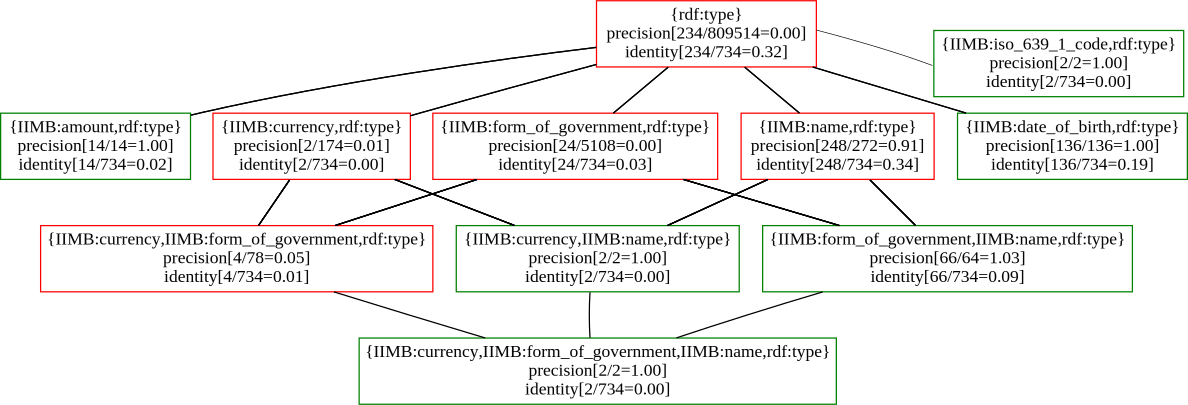
\includegraphics[width=\textwidth]{./img/iimb_16_2}
\caption{
  Example of the identity sub-relations for a given dataset (IIMB).
  Each box represents such a sub-relation.
  The lower and higher approximation are colored in green and red
    respectively.
  Each box shows the shared predicate terms in curly braces.
  The precision is calculated according to definition \ref{def:precision}.
  SECOND NUMBER
}
\end{figure*}

The approach outlined in section \ref{sec:approach}
  allows us to calculate the sub-relation hierarchy of
  a given identity relation.
Figure \ref{fig:ihierarchy} shows an example of the lower and higher
  approximations for a data- and linkset combination of the IIMB database.
Each rectangular box represents an identity sub-relation.
Since in this figure a partition is only drawn when there is at least one
  identity pair that is indiscernible with respect to some set of
  predicates, the higher approximation amounts to the entire figure.
The lower approximation only consists of those partition sets that contain
  at least one identity pair, and that contain no non-identity pair;
  these are distinguished by green borders.
For each box the precision has been calculated
  according to definition \ref{def:precision}.

\begin{definition}[Precision]
\label{def:precision}
The precision of an identity sub-relation is
\[
  \frac{
    \text{The number of identity pairs in the sub-relation}
  }{
    \text{The number of pairs in the sub-relation}
  }
\]
\end{definition}

From this definition it is clear that
    sub-relations in the lower approximation have precision $1.0$
  and that
    sub-relations in the higher approximation have a precision
      between $0.0$ and $1.0$ (exclusive).



\subsection{Applications}
\label{sec:applications}

Based on the partition of the identity relation and the set of all pairs,
  a characterization can be given of the identity relation
  and sub-relations can be distinguished (see figure \ref{fig:ihierarchy}).
If we also use the precision of each partition member,
  we can also give suggestions about pairs that may be interesting candidates
  for inclusion in or exclusion from the identity relation.

Alternatively, a low precision may indicate that objects are not
  discernible in terms of the currently asserted predicates.
This is also a relevant form of feedback,
  since if a modeler has though of two objects as being identical
  without them sharing any properties, ...

This often happens when the (natural language) contents of non-typed labels
  are used in order to characterize objects.
For example, two objects that have 

Finally, the difference between higher and lower approximation
  gives an indication of the quality of the identity relation.



\subsection{Implementation}
\label{sec:implementation}

% INTRO
In order to evaluate our approach outlined in section \ref{sec:approach}
  we implemented an algorithm that calculates
  the discernibility partition, rough set approximation and quality,
  for RDF data that containing identity statements.\footnote{
      % ALIGNMENT
      Identity statements are either loaded from a VoID-described
        linkset \cite{Void2011}
        or are loaded from an alignment file that are formatted in
        EDOAL (Expressive and Declarative Ontology Alignment Language)
        \cite{DavidEzenatScharffeTrojahn2011}.
    }
The implementation built for this paper is deployed as an extension pack
  of the ClioPatria triple store \URL{cliopatria.swi-prolog.org}.\footnote{
      The code is disseminated at \URL{github.com/wouterbeek/IOTW/}.
      % PROLOG,GRAPHVIZ,AJAX
      GraphViz is used for visualizing the hierarchy of
        identity sub-relations.
      % MATERIALIZATION
      For materializing the graph under RDFS and OWL entailment,
        we use Jena 2.11.0 \cite{Carroll2004}.
    }

% COMPLEXITY: EASY
Since in real-world data the number of identity pairs
  is relatively small when compared to the number of possible pairs,
  calculating the predicate sets that characterize higher approximation
  sub-relations is cheap.
Even calculating this using the path-expressions extension
  (section \ref{sec:generalized_predicates})
  is cheap, since the number of edge types in RDF data is relatively big
  (so there are not many sequences of identical predicates).
It is also cheap to calculate the predicate sets that characterize
  the lower approximation, plus its extensions,
  since there are relatively few sub-relations that belong to it,
  and most such sub-relations have a relatively small extension.

% COMPLEXITY: DIFFICULT
It is more costly to calculate the extension of the sub-relations that are
  in the higher approximation (and that are not in the lower approximation).
This requires an inverse search, starting from sets of
  indiscernibility predicates, and ending with (identical and non-identical)
  pairs of objects sharing (all and only) those predicates.
The extension of sub-relations is, however, necessary in order to
  calculate the quality of the identity relation
  as well as the precision (definition \ref{def:precision})
  of each sub-relation.
Since these metrics are useful for the applications outlined
  in section \ref{sec:applications},
  we want to optimize these calculations.
For briefly describe three such optimizations.

% (1) QUERY OPTIMIZATION
Firstly, we optimize the search by restricting the number of pairs
  for which we have to check whether they share a given set of predicates.
We do this by ordering the predicates based on their
  estimated complexity \cite{Wielemaker2005},
  allowing us to match triples that contain rarely occuring predicates
  before matching frequently occuring predicates.
Additionally, by using an arbitrary strict order on terms
  (e.g. lexicographically),
  only half the search space needs to be taken into account
  due to the symmetric nature of equivalence.

% (2) DATASCRUTURES
Secondly, we use an AVL tree-based association list
  in order to store the indiscernibility predicates.
The storage of indiscernibility properties uses a similar, but nested
  association list (mapping sets of predicate terms onto
  maps from sets of object terms onto sets of subject term pairs).
This means that operations on datastructures are at most $O(\log(n))$.

% (3) XML DATATYPES: CANONICAL FORM
Thridly, it is expensive to determine whether lexical expressions
  of the same datatype are identical or not,
  due to time spent on parsing those expressions
  in order to determine their value.
In the worst case. the number of such parses is quadratic
  in the number of same-typed literals.
Since canonical mappings are one-to-one \cite{XmlSchema2012},
  it is possible to determine value identity based on
  canonical lexical expression comparison,
  requiring only a linear number of lexical expression parses.
This is acchieved by converting all lexical expressions
  to their canonical lexical form prior to running the main algorithm.

\begin{comment}
Existing SW libraries implement equivalence relations for common datatypes,
  but equivalence is not always in line with identity.
Therefore, exceptions have to be made for specific values
  that are known to have equivalent non-identities (such as $0$ and $-0$)
  and non-equivalent identities (such as $NaN$ for {\small \texttt{float}}).
The latter even provides a rare instance of violating the common definition
  of identity as the smallest equivalence relation.
\end{comment}

\section{Experimental design}
\label{sec:experimental_design}

For illustrative purposes we use the IIMB dataset that is used in the
  instance matching track of the 2012 Ontology Alignment Evaluation
  Initiative (OAEI\footnote{\URL{oaei.ontologymatching.org}}).
This dataset consists of eighty ontologies $G_i$ (for $1 \leq i \leq 80$)
  that are linked to a single base ontology $G_0$.
The identity links between $G_0$ and $G_i$ are annotated with a
  confidence measure between $0.0$ and $1.0$.
A graph $G$ is the result of fully materializing the graph merge
  of $G_i$ (for some $1 \leq i \leq 80$) and $G_0$.
For each of these eighty linked ontologies a reference mapping is available.



\subsection{Experimental results}

In this experiment we incrementally remove part of the identity relation.
We then calculate the rough set representation using this altered relation.
We then evaluate how many of the removed identity pairs occur in
  the higher approximation.
Our hypothesis is that the percentage of removed identity pairs
  in the higher approximation is higher than the percentage of pairs
  in the higher approximation.
If the hypothesis is validated, this indicates that
  calculating the rough set representation for a partial identity relation
  would indeed improve suggestions for extending that identity relation.

Since the data may contain noise, using precision degrees $0.0$ and $1.0$
  may be too strict. For this experiment we have set these boundaries
  to $0.05$ and $0.95$ respectively.

\begin{figure}
\label{fig:recall_quality}
\centering
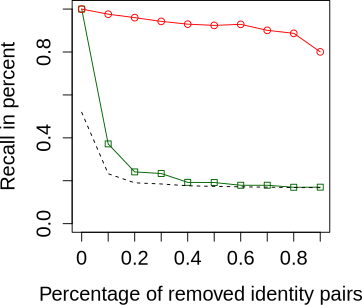
\includegraphics[width=0.8\linewidth]{./img/recall_quality}
\caption{
  The recall of the lower and higher approximation
    are shown by the green and red line respectively.
  The quality metric (definition \ref{def:quality})
    is shown by the dashed line.
}
\end{figure}

\begin{figure}
\label{fig:in_higher}
\centering
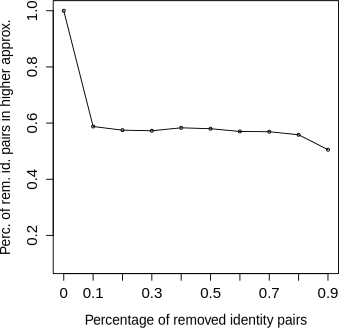
\includegraphics[width=0.8\linewidth]{./img/in_higher}
\caption{
  The percentage of the removed identity pairs that are in the higher approximation
}
\end{figure}

In figure \ref{fig:in_higher}
  we see that the randomly removed identity pairs are often
  in the higher approximation, even when large parts of
  the identity relation are removed.

\begin{comment}
Lower recall
1.0,0.37172100183246687,0.24123550044617229,0.23375413992878838,0.19251810221158194,0.1916729296953922,0.1790536768898471,0.17912482945205316,0.1696252362320524,0.17011849853438268
Higher recall
1.0,0.976185052819561,0.9600384749021372,0.9425765362723856,0.9297564861502547,0.9239282325982691,0.9288077551757412,0.900878631549093,0.886987450993775,0.8005503359226204
Quality
0.5190405227795084,0.23261438049447705,0.1904353344556299,0.18505145463363135,0.17658153004935476,0.17387635867899948,0.17168948193128328,0.17017370794837366,0.16844506704419984,0.1677780567227606
Higher cover
0.0006413304103753317,0.0006098495555258293,0.0005825544051162525,0.0005747252831024628,0.0005640718998200667,0.0005626590987592347,0.0005613753926606205,0.0005464403973849621,0.0005372610299329459,0.00046916805031848495
Removed identity pairs in higher
1.0,0.5877680311890837,0.5747530425162004,0.572660333493667,0.5831761670185315,0.5799385908868745,0.5701984042084377,0.5692284399224807,0.558405393333526,0.5051324217787632
\end{comment}


\subsection{Hypotheses}
\label{sec:hypotheses}

Since this paper focusses on our novel approach and not on evaluation,
  we will enumerate some of the hypotheses which can be evaluated
  using the here described approach:
\begin{enumerate}
\item Take an {\small \texttt{owl:sameAs}} relation and
        a {\small \texttt{skos:related}}
        relation defined over the same domain.
      Merge them into a new binary relation $\sim$.
      Establishing the lower and higher approximation of $\sim$,
        the hypothesis is that pairs from {\small \texttt{owl:sameAs}}
        occur more frequently in the lower boundary than pairs from
        {\small \texttt{skos:related}},
\item Take a set of alignment pairs, each of which is associated with
        a confidence measure between $0.0$ and $1.0$.
      Choose an arbitrary cutoff point $0.0 < c < 1.0$.
      The hypothesis is that alignments with a confidence larger than $c$
        occur more frequently in the lower approximation than alignments
        with a confidence smaller than $c$.
\item Take a set of automatically generated alignment pairs with
        associated confidence measures and take the gold standard or
        reference alignment for the same dataset.
      The hypothesis is that pairs that occur in the lower approximation
        of the alignment appear relatively more often in the gold standard
        than pairs that occur in the higher approximation of the alignment.
\item The quality measure $\alpha$ of a reference alignment is generally
        higher than the accuracy measure of an automatically generated
        alignment for the same dataset.
      Or, the quality measure is generally higher for identity relations
        that domain experts consider to be correct.
\end{enumerate}

Also, the IIMB datasets are quite small (tens of thousands of triples).
We will have the verify whether the current implementation is able to scale
  to bigger datasets.


% Section 4: Conclusion
\section{Conclusion}
\label{sec:conclusion}

In this paper we have given an new approach for characterizing,
  extending/retracting, and assessing identity relations.
Our approach does this in purely qualitative terms, using schema semantics.
In contemporary ontology alignment and data linking activities nonsemantic
  aspects of resources play a role as well.
For instance similarity assessment for natural language labels is often
  used in data linking.

We think that the qualitative means of characterizing an identity relation
  are a useful addition to existing quantitative means.
Also, we think that it is more useful and viable to enrich existing
  identity relations in the LOD based on the semantics of the datasets
  in which they occur, than to introduce new relationships into SW languages.
Apart from the practical difficulties of teaching practitioners
  and transforming/enriching existing datasets, we suggest that the
  meaning of an identity (sub)relation is partially defined in its use,
  i.e., in the indiscernibility criteria it embodies.

For our approach it is not necessary to pose additional restrictions
  on a binary relation $\sim$.
The definitions in this paper apply to \verb|owl:sameAs| relations
  in the same way in which they apply to any other binary relation
  (e.g., \verb|skos:related|).

We are currently in the process of validating the above enumerated hypotheses.
The results of these evaluations are continuously being published on
  \verb|wouterbeek.com/identity-on-the-web|.
The website currently contains the automated results of all eighty IIMB
  alignments, drawn from the instance matching track of the
  OAEI 2012.
The website also refers to the publicly available Git repository
  \verb|github.com/wouterbeek/IOTW| where the implementation
  discussed in section \ref{sec:implementation} can be found.

%\input{./tex/futurework.tex}

% Bibliography
\bibliographystyle{aaai}
\bibliography{iotw,prasem,web_standards}

\end{document}

